\documentclass[10pt, a4paper,titlepage]{article}

\usepackage{graphicx}
\usepackage{listings}
\usepackage[normalem]{ulem}
\usepackage{caption}

\begin{document}
\begin{titlepage}
\title{Design Document \\Version 1.0}
\author{Emanuele Ricciardelli (mat. 875221) \and Giorgio Tavecchia (mat. 874716) \and Francesco Vetr\'o (mat. 877593)}
\begin{figure}
\begin{center}

\includegraphics{/home/francesco/git/Project_SE2_RTV/DD/DD_images/logopolimi.png}
\caption{Politecnico di Milano}
\label{fig:logo}
\end{center}
\end{figure}
\maketitle
\end{titlepage}
\tableofcontents
\pagebreak
\section{Introduction}
\subsection{Purpose}
This document will provide a set of architectural and design details in order to drive software developent of the PowerEnjoy system-to-be. Specifically,  the following will be now identified and described:
\begin{itemize}
\item High level architecture;
\item Main component view;
\item The runtime behaviour of components;
\item Design patterns.
\end{itemize}•
\subsection{Scope}
The system should be able to register new users with their credentials, such as name, surname, address and e-mail, their valid driving license number and some payment information. Once the registration process is completed and all entered data are verified, the system will send a password to the user: this password will be used by the user to access the system and its functionalities. The system provides the following common features: 
\begin{itemize}
\item find an available car;
\item reserve an available car one hour prior the pick up; 
\item unlock the car when the user is detected nearby the car he/she reserved;
\end{itemize}•
In addition there will be incentives for virtuous behaviors of the user that will affect their fares: if an user helps the community by being responsible with the usage of the car, his/her fare will be reduced by a specified percentage; otherwise, by not following the guidelines of the company, the user will be charged more than the standard fare
\subsection{Definitions, acronysm, abbreviations}
\begin{itemize}
\item \underline{\textbf{RASD}}: Requirements Analysis and Specifications Document;
\item \underline{\textbf{Gateway}}: tool to set the communication and the exchange of data between two or more networks with, often, different protocols;
\item \underline{\textbf{Push notification}}: notification sent to a smartphone via application installed on it;
\item \underline{\textbf{Email}}: mail service carried over the web;
\item \underline{\textbf{API}}: Application Programming Interface.  It is a set of subroutine definitions, protocols, and tools for building application software;
\item \underline{\textbf{Google Maps API}}: APIs provided by Google to compute functionalities over the Google Maps environment;
\item \underline{\textbf{MVC}}: Model View Controller pattern;
\item \underline{\textbf{Tier}}: architectural level in which the system is decomposed;
\item \underline{\textbf{Client}}: program or part of a program which allows to exchange data with a server to perform computations;
\item \underline{\textbf{Thin Client}}: client dedicated to only graphical representation, which displays the results of a computational logic contained exclusively in server;
\item \underline{\textbf{Application Server}}: it provides the infrastructure and support functions, development and execution of applications in a distributed environment;
\item \underline{\textbf{Database Server}}: software system able to store and manipulate data contained in a database;
\item \underline{\textbf{Execution Environment}}: it represents a particular execution platform, such as an operating system or a database management system. Execution environments are used to describe the context in which the execution of a model takes place;
\item \underline{\textbf{Controller}}: software system that applies changes to the model and database;
\item \underline{\textbf{UX}}: user experience diagram;
\item \underline{\textbf{BCE}}: Boundary Control Entity diagram;
\item \underline{\textbf{Ticket}}: the term refers to a fine that a driver has received during a ride;
\item \underline{\textbf{Record Maintenance}}: record saved in the Database, used to save information concerning the maintenance processes of a car.
\end{itemize}•
For all terms not specified, please refer to the glossary contained in the previous document (RASD).
\subsection{Reference documents}
\begin{itemize}
\item Specification document: Assignments AA 2016-2017.pdf;
\item RASD previously version 1.0;
\end{itemize}•
\subsection{Document structure}
\begin{itemize}
\item Introduction: this section introduces the design document, providing a brief indication of its utility and about the covered sections;
\item Architecture design:
\subitem - Overview: this sections explains the high level components and their interaction;
\subitem - Component view: more detailed view of the components of the application;
\subitem - Deployment view: this section shows all components that must be deployed to have the application running completely and correctly;
\subitem - Runtime view: it describes how components interact with each other to accomplish specific tasks;
\subitem - Component interfaces: it describes the interfaces between the components;
\subitem - Selected architectural styles and patterns: it provides details related to patterns and architectural styles selected for the development;
\subitem - Other design decisions;
\item Algorithms design: this section provides some algorithms useful to describe some functionalities of the system;
\item User interface design: this section presents a detailed description of user experience explained with diagrams like UX and BCE;
\item Requirements traceability: this section aims to explain how the decision taken in the RASD are linked to design elements.
\end{itemize}•
\newpage
\section{Architectural Design}
\begin{figure}
\includegraphics[scale=0.4, keepaspectratio]{/home/francesco/git/Project_SE2_RTV/DD/DD_images/High_level_components.png}
\caption{High level components}
\label{fig:high_level_components}
\end{figure}
\subsection{Overview}
The PowerEnJoy system will be shaped in a three tier architecture. This architectural style allows a further enhancement: the possibility to move the entire application in a dedicated cloud server with elastic infrastructure in order to get performances needed by the load on the application on demand and the consequent money saving. This choice will also face the coupling problem with respect either to the logic and data level and to the logic and presentation level. Nonetheless a performance evaluation might need to check whether the contract terms are satisfied. Important decision based on this architecture is the thin client characterization: the client can only send to the server a sequences of requests on what operation is intended to perform. This choice can possibly raise the expenses for the company. In the right part of Figure 2 is present the component named as “Payment System”: this component is intended to be a set of functionalities offered to the banks in order to ensure the correctness of all the payment operations. In Figure 3 we show the existence of firewalls in between the layers: this is due to the high security problems that this service arouse. Since our data level will store personal information such as identity, mail address, number of credit cards and even positions of a human being, a possible solution is to use different techniques to ensure that none will ever access private data.
\begin{figure}
\begin{center}
\includegraphics[scale=0.6, keepaspectratio]{/home/francesco/git/Project_SE2_RTV/DD/DD_images/Tier_levels.png}
\end{center}
\caption{Tier levels}
\label{fig:tier_levels}
\end{figure}
\newpage
\subsection{High level components and their interaction}
The high level components architecture in Figure 2 is made of five parts. The main part is the \emph{Global system}: it is a singleton that contains all the business logic. It is splitted into two sections: 
\begin{itemize}
\item the \emph{Car sensors subsystem}, as stated in the RASD, the cars are seen by the system as a set of sensors that only provide data. This part of the system-to-be is devoted to collect data from cars, convert them in a usable structure for the system and then send them to the business logic part named \emph{Application server};
\item the \emph{Application server} that will receive requests, will manage the information provided by the \emph{Car sensors subsystem} and will be able to communicate with the \emph{Payment system} in order to retrieve payments information.
\end{itemize}•
The customer, via the mobile app or the service’s web page, can initiate a communication with the \emph{Application server} that will complete the task requested and will answer back immediately with a message about the success or failure of the request and, if other information are needed, will send an email or a push notification providing the missing part (e.g. the client reserves a car, the request is successful and the system answers with a push notification/email containing the code to unlock the car).
Then the maintenance service can communicate with the main application by visiting a dedicated web page. Here the maintenance personnel can look at all the stored maintenance requests and change the status of this requests. (e.g. a request of a car left with less than 5\% of the battery might be changed to \textit{performing}, and after the car is put in charge its status will be changed in \textit{complete}).
In the right part of Figure 2 there is the \emph{Payment system}. This system is supposed to interact with banks and the “Application server” in order to perform checks and updates all the information regarding payments. The banks will use this interface to communicate with our system, and the \emph{Payment system} will act as a controller and will request the \emph{Application server} to perform the needed changes to the database in order to maintain the correct status of payments and users. This is due to a previous decision stated in the RASD \textit{(Table 13: Provide a payment)}.
The \emph{Application server} needs to store and perform queries in order to perform all the tasks and so communicates with a database.
\clearpage
\begin{figure}[h]
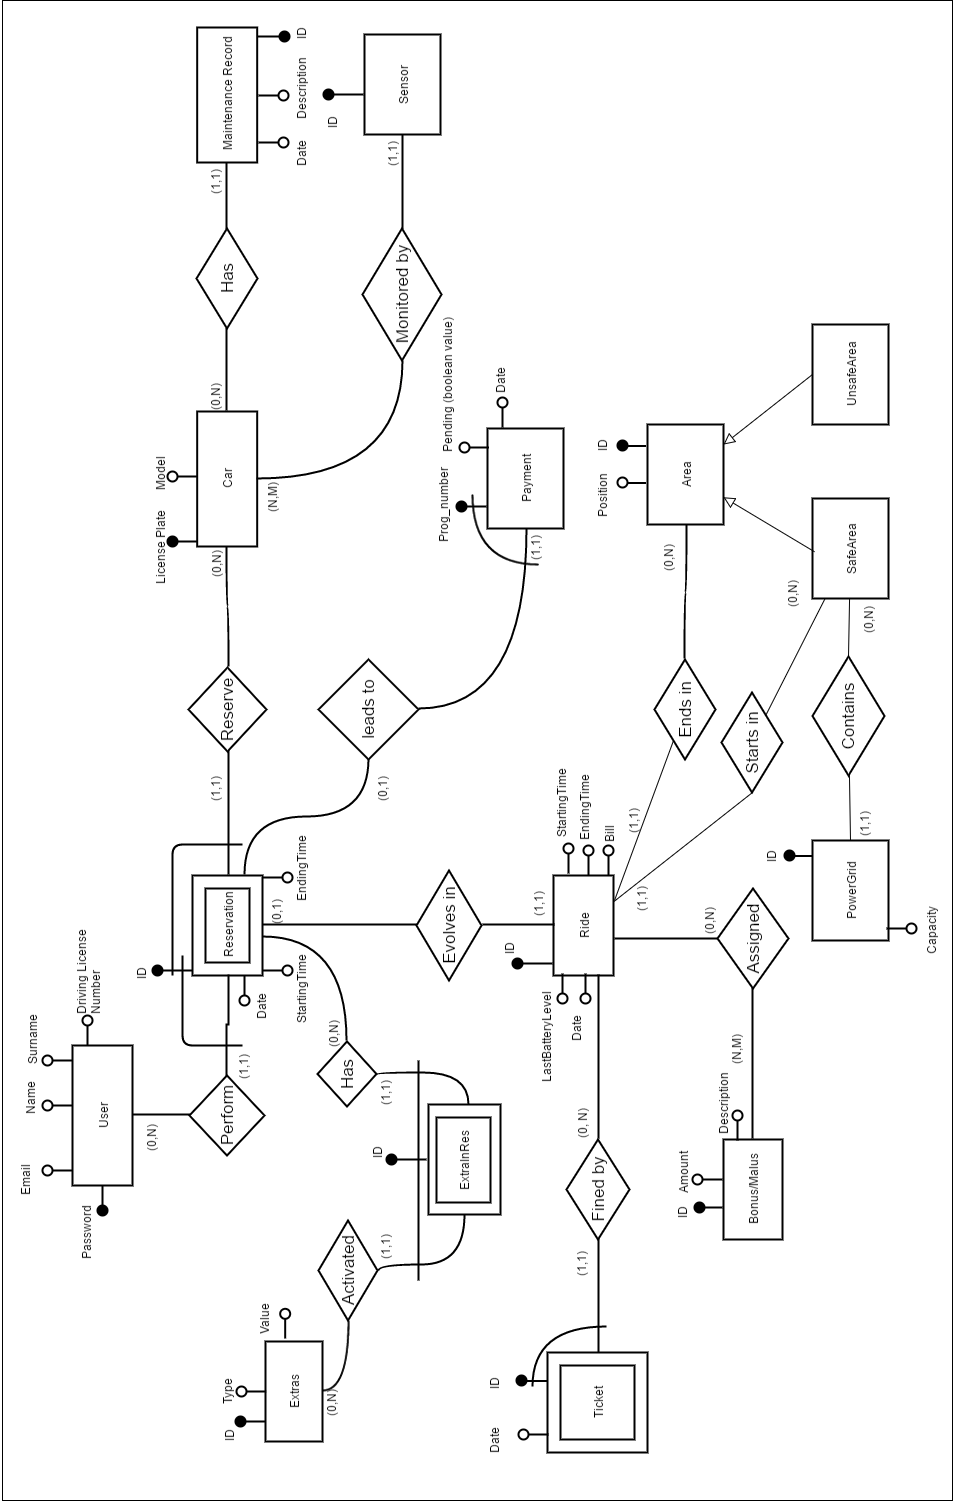
\includegraphics[width=\textwidth,height=\textheight,keepaspectratio]{/home/francesco/git/Project_SE2_RTV/DD/DD_images/ER.png}
\caption{ER diagram}
\caption*{\underline{Observation}: ID in \emph{Reservation} entity will later be converted into QR Code to enable the user to access the car that he has previously reserved.}
\label{fig:ER}
\end{figure}
\clearpage
\subsection{Component view}
\begin{figure}
\begin{center}
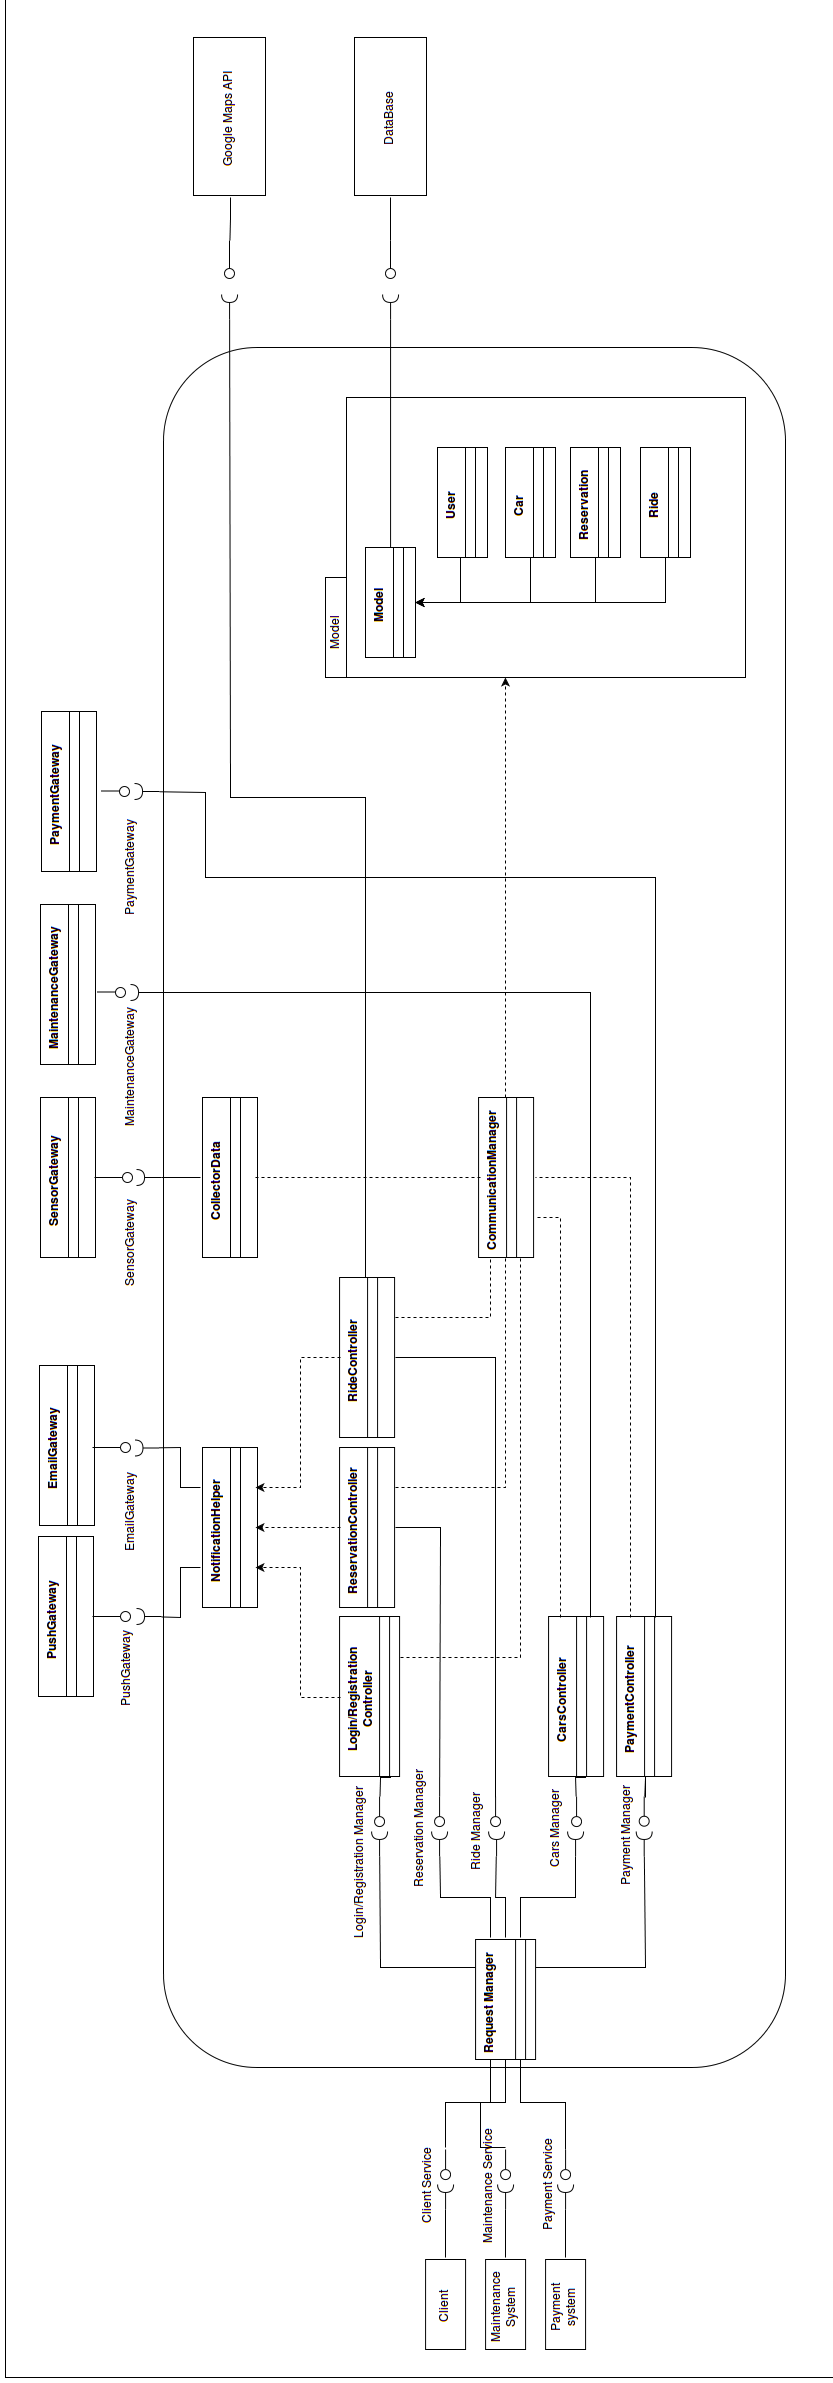
\includegraphics[width=\textwidth,height=\textheight,keepaspectratio]{/home/francesco/git/Project_SE2_RTV/DD/DD_images/Component_view.png}
\caption{Component view}
\label{fig:component_view}
\end{center}•
\end{figure}
The component view consists of the following components:
\begin{itemize}
\item \textbf{Client}: client’s device used to connect to the service
\item \textbf{Maintenance}: maintenance device used to interact with the system in order to provide maintenance features.
\item \textbf{Payment system}: third party device used to provide information about payments, their completion and other information relating.
\item \textbf{Request manager}: manager used to receive request from the outside and to route them to the correct controller. 
\item \textbf{Login/Registration controller}: manage login and registration aspects
\item \textbf{Reservation controller}: manage reservation aspects.
\item \textbf{Ride controller}: manage ride aspects.
\item \textbf{Cars controller}: manage all informations related to cars, sensors and their interaction with the users.
\item \textbf{Collector data}: manage the data collection from different sensors
\item \textbf{Payment controller}: manage payment aspects like register debts or mark their completion.
\item \textbf{Communication manager}: component used to manage information exchange between different controllers and between them and the model.
\item \textbf{Notification helper}: manage notification aspects, routing them to the correct gateway
\item \textbf{Push gateway}: manage the sending of push notification to mobile app.
\item \textbf{Email gateway}: manage the sending of Email messages.
\item \textbf{Sensor gateway}: handle the sending and receiving of data collected by the various sensors present on cars.
\item \textbf{Maintenance gateway}: manage the sending of notification to the maintenance company
\item \textbf{Payment gateway}: manage the sending of payment information to the third party payment service
\item \textbf{Model}: model of the world, used by the controllers.
\item \textbf{Database}: database used to store persistent data.
\item \textbf{Google Maps API}: API service used by the ride controller to provide navigation information.
\end{itemize}•
The interaction between the system and users is provided by a series of interfaces, one for each type of actor. All requests are handled by the single component \emph{Request Manager} that will provide for their proper forwarding within the system. We have designed a system consisting of several controllers, each dedicated to a specific type of functionality. This allows us to maintain a high level of cohesion of the different components, allowing, in case of future expansions of the service, to update the individual components smoothly and with great flexibility. The division of functions in various components will also allow us to efficiently test the service provided. In order to maintain a high degree of flexibility, we decided to introduce a component \emph{Communication manager} dedicated to the sorting of the information exchanged between the controllers themselves and the model, thus avoiding the definition of direct links between controllers that might obstruct and make more complex a future possible expansion of the service.
In analogous way we introduced a component \emph{Notification helper} dedicated to the proper addressing of the notifications to users, thus separating the functionality of sending of notifications from the logic of the underlying service.
As shown in the diagram, the only access to the model and to the database it is via the \emph{Communication Manager} that will carry out read and write functionality.
\newpage
\subsection{Deployment view}
\begin{figure}[h]
\begin{center}
\includegraphics[width=\textwidth, height=0.7\textheight, keepaspectratio]{/home/francesco/git/Project_SE2_RTV/DD/DD_images/Deployment_view.png}
\caption{Deployment view}
\label{fig:deployment_view}
\end{center}•
\end{figure}
\newpage
\subsection{Runtime view}

\enddocument